\chapter{Proposta de Ferramenta}

Nesta seção, será apresentada uma ferramenta cujo objetivo é automatizar a geração de questões, com o objetivo de tornar mais fácil a construção e geração de questões. A ferramenta baseia-se em um modelo de separação entre duas entidades principais : (i) um JSON de template, responsável por definir a estrutura geral das questões; e (ii) um JSON de questões, que instancia as variações específicas de cada problema. O sistema foi planejado para permitir que os professores sejam responsáveis pela elaboração e manutenção dos templates. Por outro lado os usuários estudantes interagem apenas com as questões geradas a partir desses templates.

\section{JSON de Templates}

O primeiro componente é o JSON de Template, ilustrado na Figura \ref{fig:json-de-templates}, no qual o enunciado geral (\textit{cabeçalho}) descreve a estrutura padrão que será aplicada em todas as questões derivadas. Nele, é definido as partes fixas do enunciado e a forma como os elementos variáveis serão combinados para formar a questão. Em seguida, cada categoria de variáveis contém uma lista de opções textuais ou numéricas que podem assumir diferentes valores de acordo com a necessidade, permitindo a criação de múltiplas versões de um mesmo problema.


\begin{figure}[ht]
	\centering
	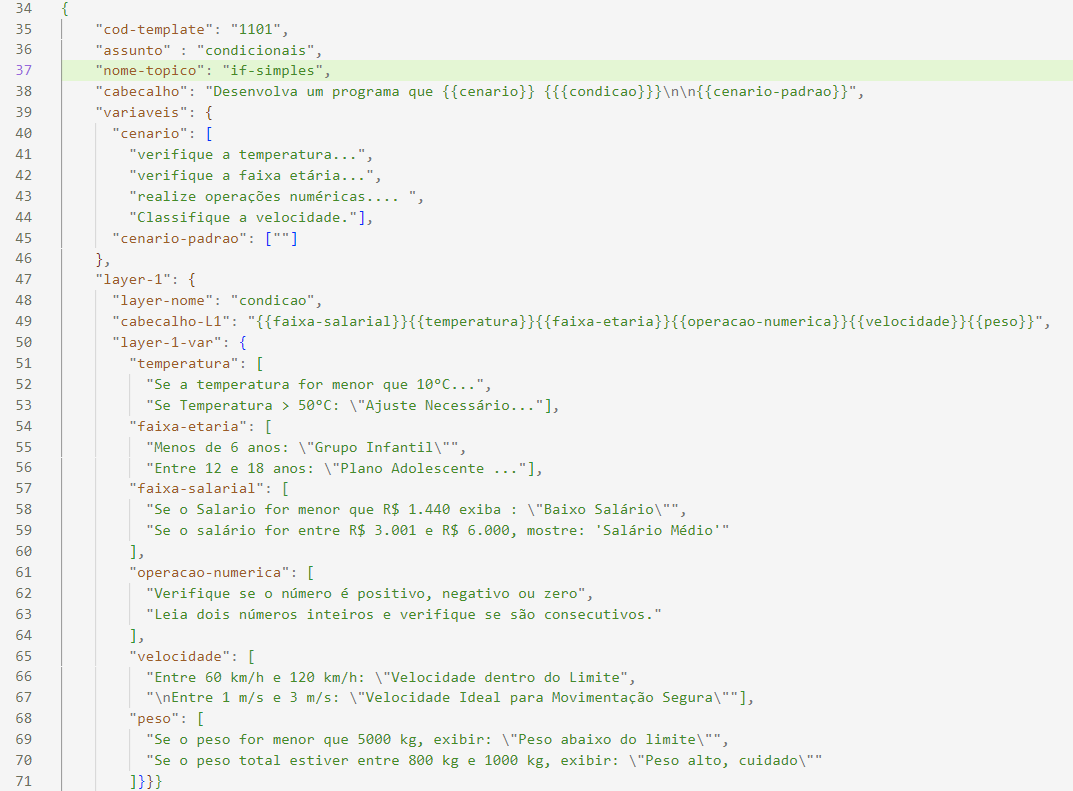
\includegraphics[width=16cm]{./imagens/capitulo7/json-de-template}
	\caption{JSON de Templates (Elaboração própria, 2025) }
	\label{fig:json-de-templates}
\end{figure}
\section{JSON de Questões}

O segundo componente é o JSON de Questões, ilustrado na figura \ref{fig:json-de-questoes}, cujo objetivo é definir o formato final de cada questão que será efetivamente apresentado aos estudantes. Neste arquivo, cada questão é identificada por um código, um título e um mapeamento dos índices das variáveis que aponta para as categorias estabelecidas no template. Assim, essa estrutura não precisa carregar toda formatação do template, apenas fazer referência aos elementos já definidos no arquivo de templates. Dessa forma, não é necessário carregar toda formatação do enunciado em cada questão, mas apenas fazer referencia ao índice dos elementos definidos do JSON de Templates. Essa separação favorece a reutilização do mesmo modelo em diversas situações, bastando alterar os atributos de cada problema conforme necessário.

\begin{figure}[ht]
	\centering
	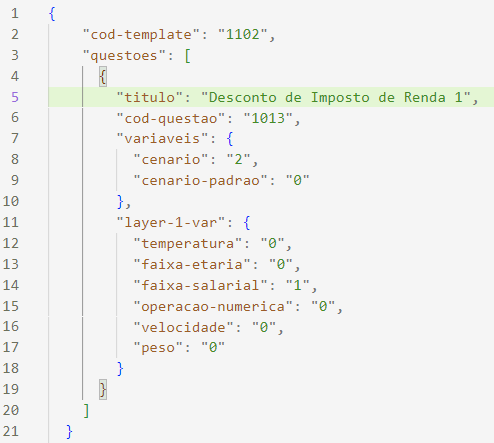
\includegraphics[width=12cm]{./imagens/capitulo7/json-de-questoes}
	\caption{JSON de Questões (Elaboração própria, 2025) }
	\label{fig:json-de-questoes}
\end{figure}
Na próxima seção serão discutidos os aspectos de implementação, apresentando a ferramenta utilizada e como a geração de questões pode ser aplicada na prática, como os dados dos arquivos JSON são processados para gerar as questões, bem como um panorama geral do sistema e detalhes do \textit{prompt} utilizado pela IA.

\section{Ferramenta}

Segundo \parencite{martin2017} a arquitetura de software deve apresentar o domínio do sistema, e não somente dos \textit{frameworks} ou tecnologias empregadas. Partindo desse princípio, a figura \ref{fig:modelo-arquitetural} organiza o sistema em quatro camadas : Apresentação, Aplicação, Domínio e Infraestrutura — de forma que reflita a descrição do fluxo quando o sistema é executado.

\begin{figure}[ht]
	\centering
	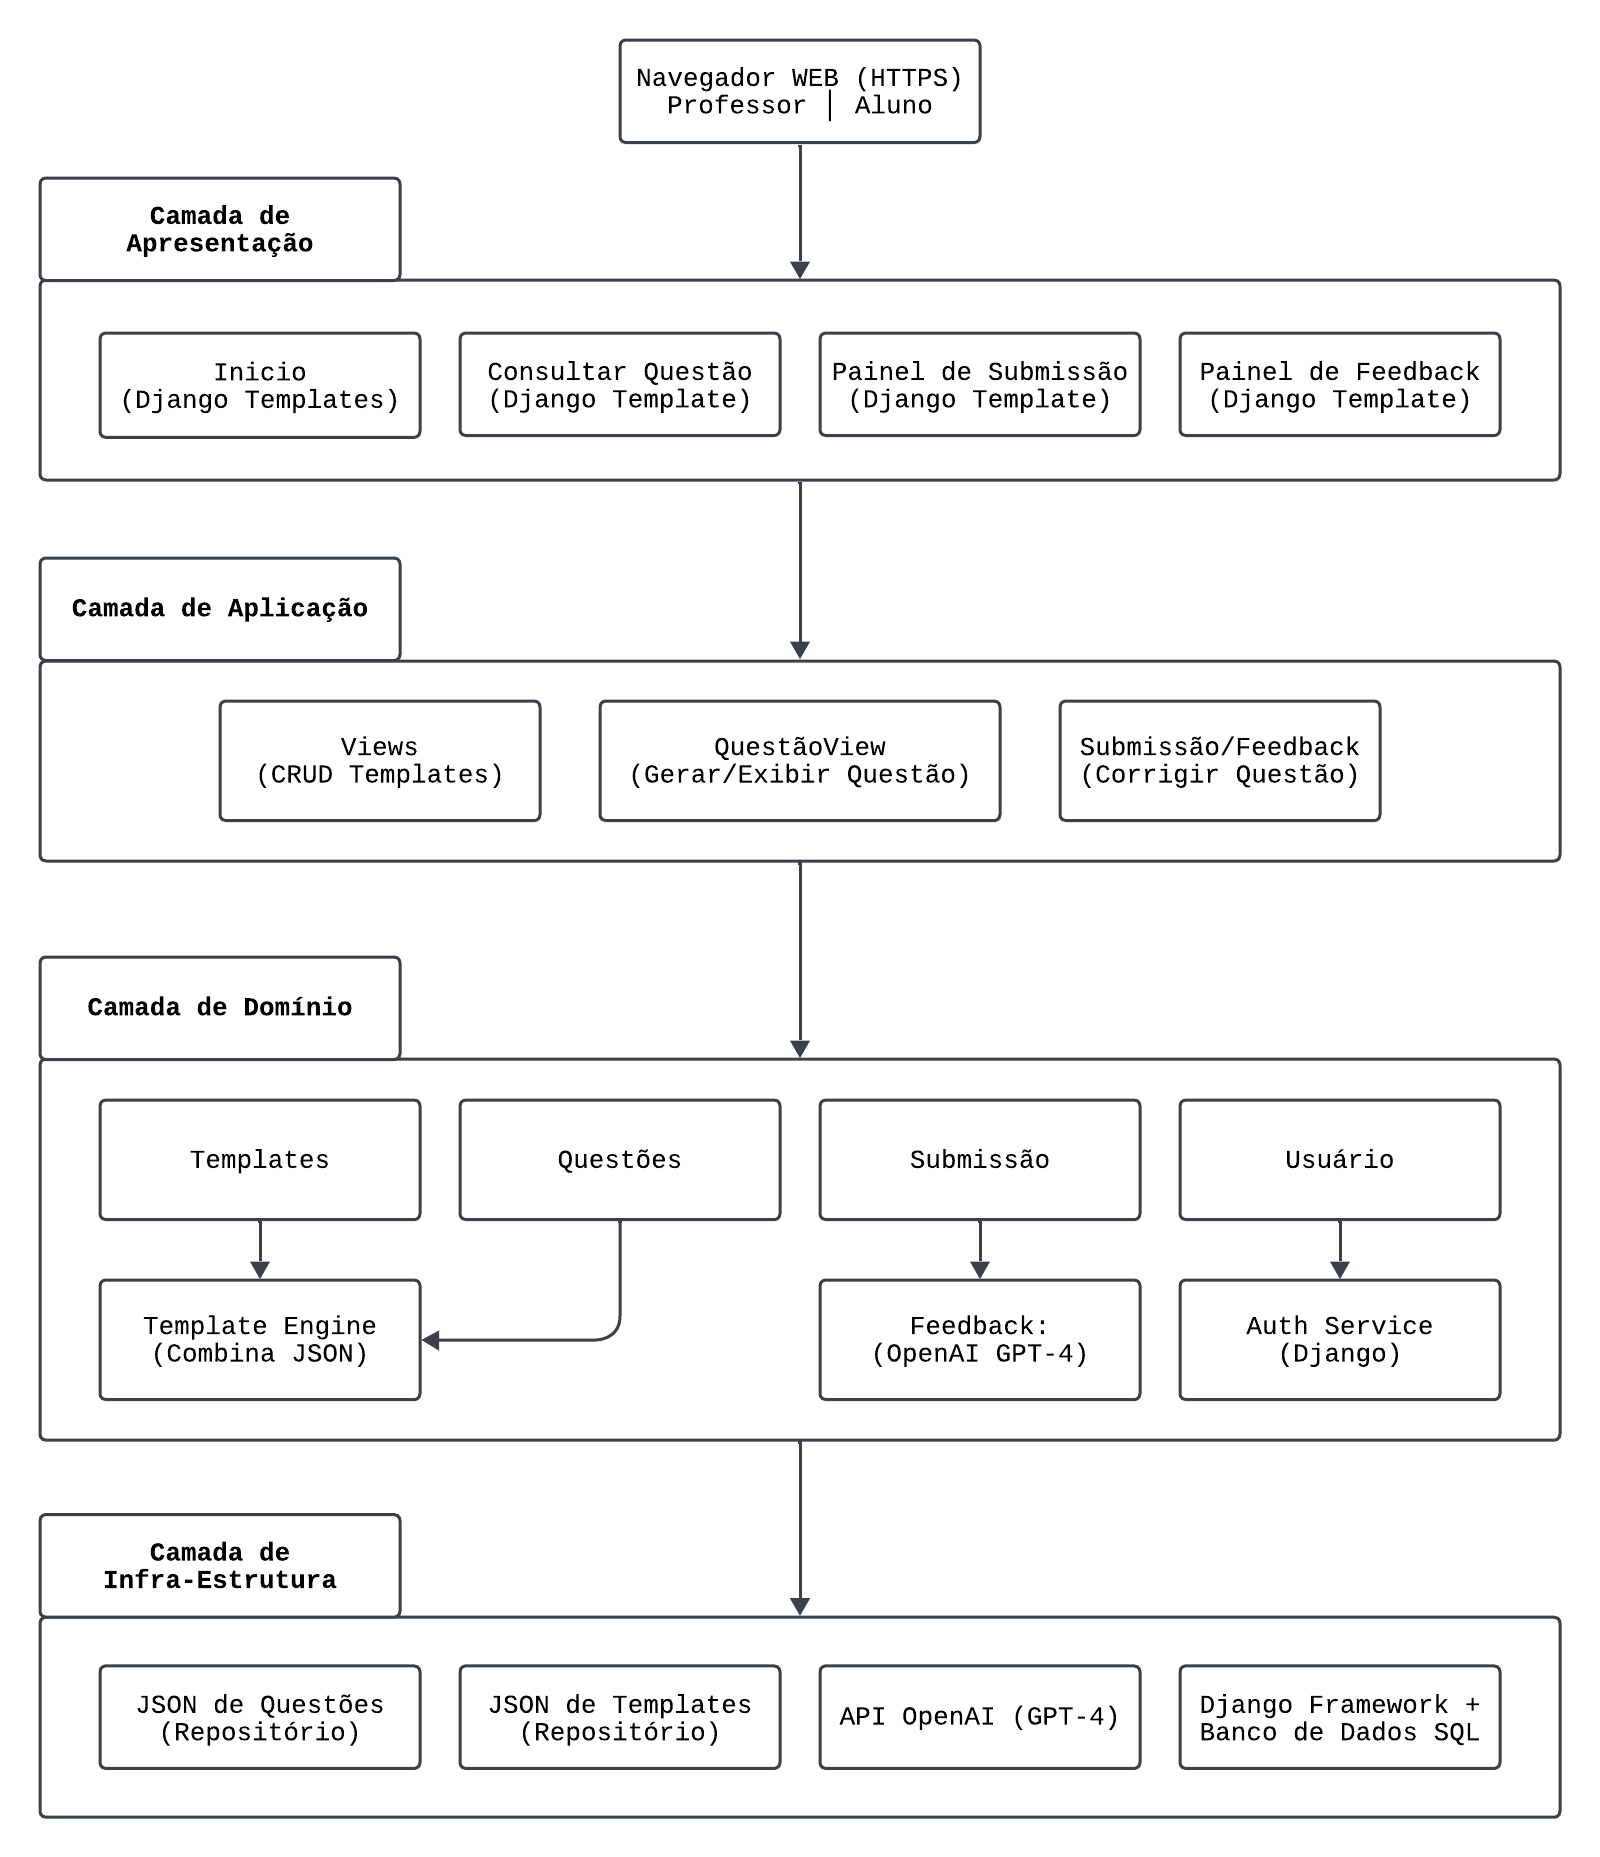
\includegraphics[width=12cm]{./imagens/capitulo7/modelo-arquitetural}
	\caption{Modelo arquitetural do sistema (Elaboração própria, 2025) }
	\label{fig:modelo-arquitetural}
\end{figure}



A ferramenta utilizada foi o \textit{Arena Code}, desenvolvida pelo autor desta pesquisa para a geração automática de questões de programação. O código-fonte da aplicação encontra-se disponível nas referências \parencite{arena-code}.
As figuras a seguir ilustram o ciclo de uso da ferramenta, no qual cada interface exerce funções específicas em diferentes momentos da interação entre o usuário e o sistema. A janela da página inicial, apresentada na Figura \ref{fig:modelo-arquitetural}, exibe uma síntese dos templates disponíveis : assunto, dificuldade e número total de combinações geradas. 
Ao selecionar um assunto de interesse, como por exemplo estruturas condicionais na Figura  \ref{fig:ferramenta-topicos}, o sistema gera dinamicamente uma questão relacionada ao tema escolhido. Essa geração é basada em um template multicamadas, que permite combinar diferentes cenários dentro de uma mesma tabela, ou utilizar mútilas tabelas para um único cenário. Essa abordagem amplia consideravelmente a quantidade de variações possíveis para uma mesma estrutura de template. 
\begin{figure}[H]
  \centering
  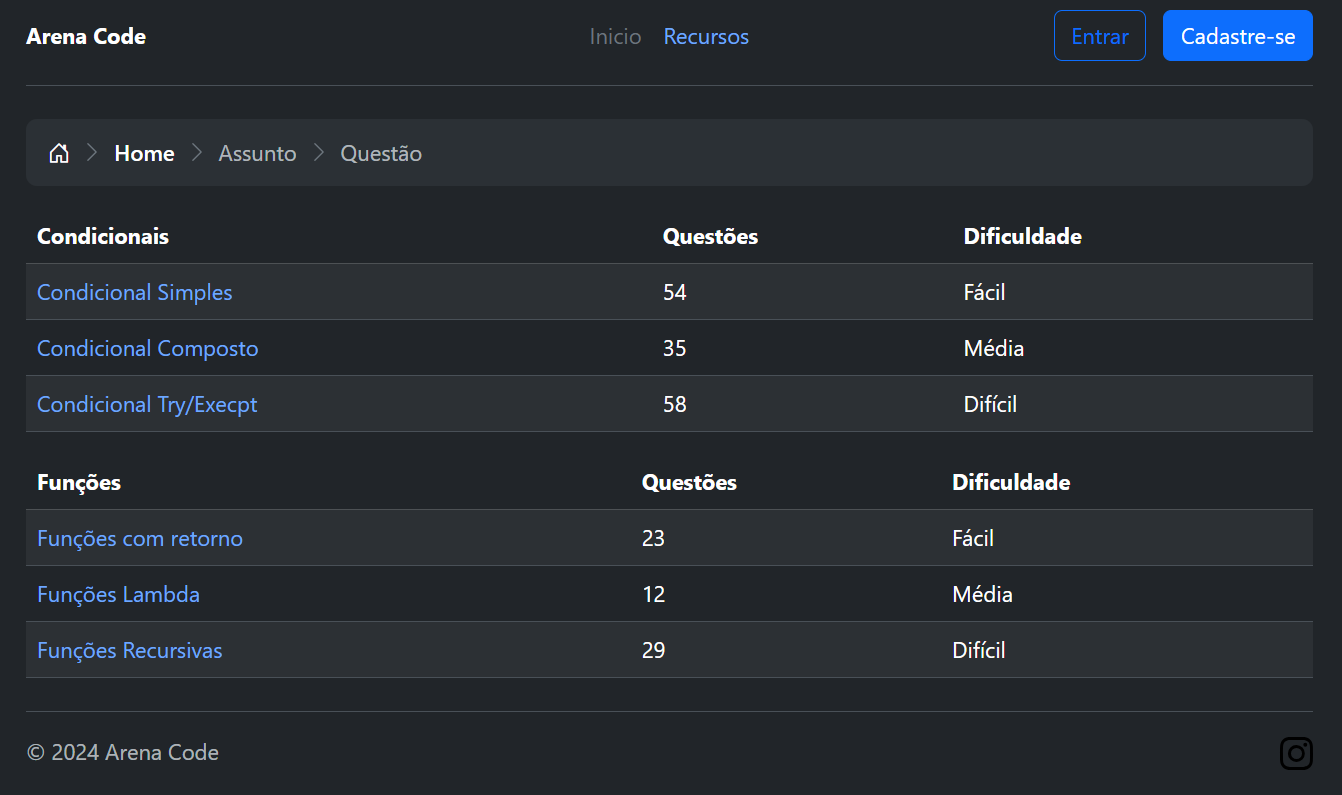
\includegraphics[width=\textwidth]{./imagens/capitulo7/ferramenta-fig1}
  \caption{Página inicial com lista de assuntos (Elaboração própria, 2025)}\label{fig:ferramenta-topicos}
\end{figure}


O processo tem início com a seleção de um template que reúne uma lista de variações previamente estruturadas. A partir dessa escolha, o sistema combina os elementos correspondentes e gera dinamicamente uma questão, que é apresentada ao aluno na página seguinte conforme a Figura \ref{fig:ferramenta-enunciado}.  Na página do enunciado, a esquerda será exibido a questão gerada de acordo com o assunto do template selecionado, e à direita é exibido o editor de código, onde o estudante deve escrever a solução proposta e posteriormente acionar o botão \textbf{submeter código}, o aluno será redirecionado para página de feedback. 

\begin{figure}[H]
  \centering
  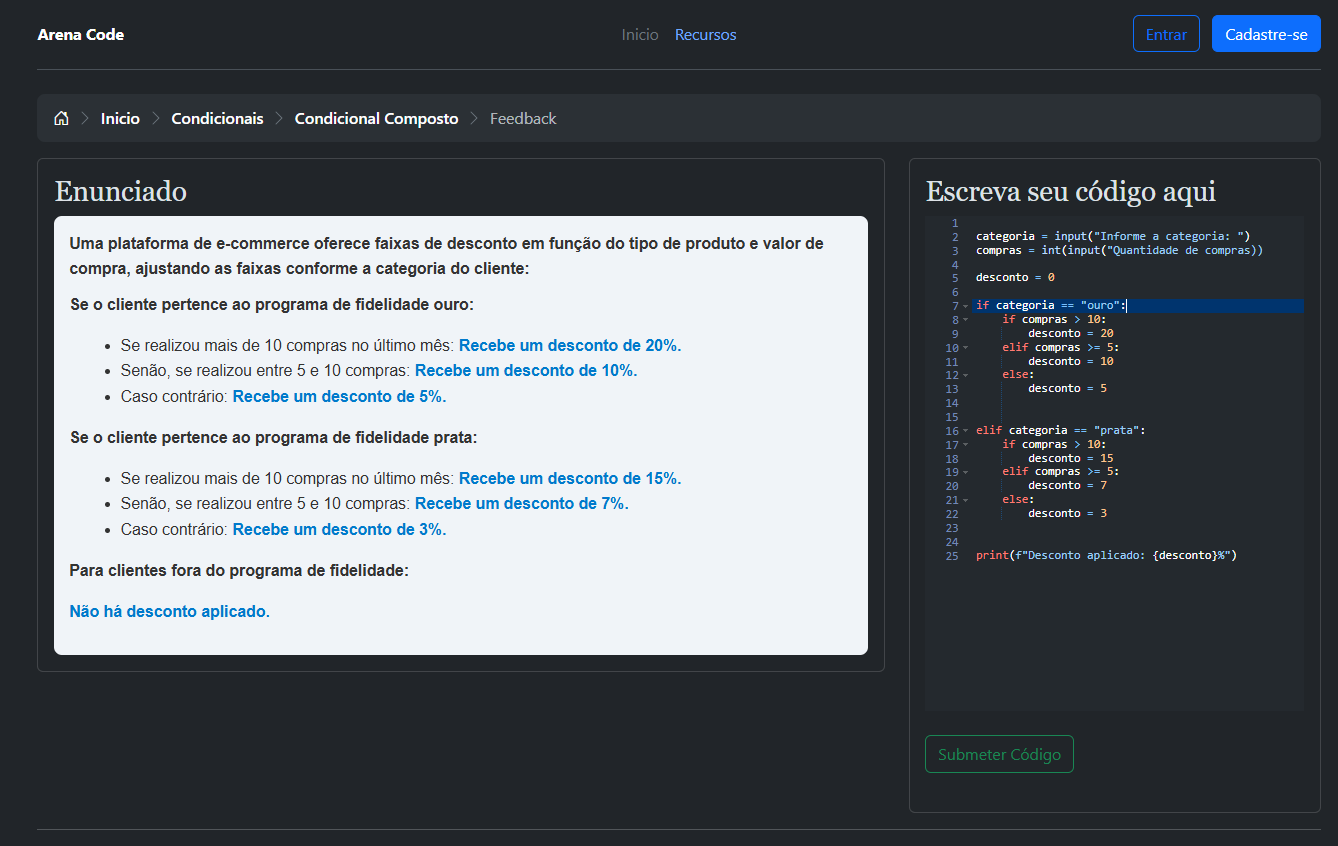
\includegraphics[width=\textwidth]{./imagens/capitulo7/ferramenta-fig2}
  \caption{Tela de resolução: Enunciado e editor de código.  (Elaboração própria, 2025)}\label{fig:ferramenta-enunciado}
\end{figure}

A flexibilidade desse template faz com que seja possível criar muitas variações de exercícios, cada um abordando aspectos distintos das estruturas condicionais. Em seguida, o código escrito no ambiente de resolução oposto e submetido para avaliação. Para realizar a correção, a ferramenta usa uma \gls{api} da OpenAI, que utiliza o GPT-4 para verificar os casos de teste associados ao problema e devolve um feedback  sobre a resposta enviada. Essa estratégia incentiva o aprimoramento constante do aluno, pois o mesmo pode corrigir e reenviar sua solução quantas vezes forem necessárias até alcançar o resultado desejado. 

\begin{figure}[ht]
	\centering
	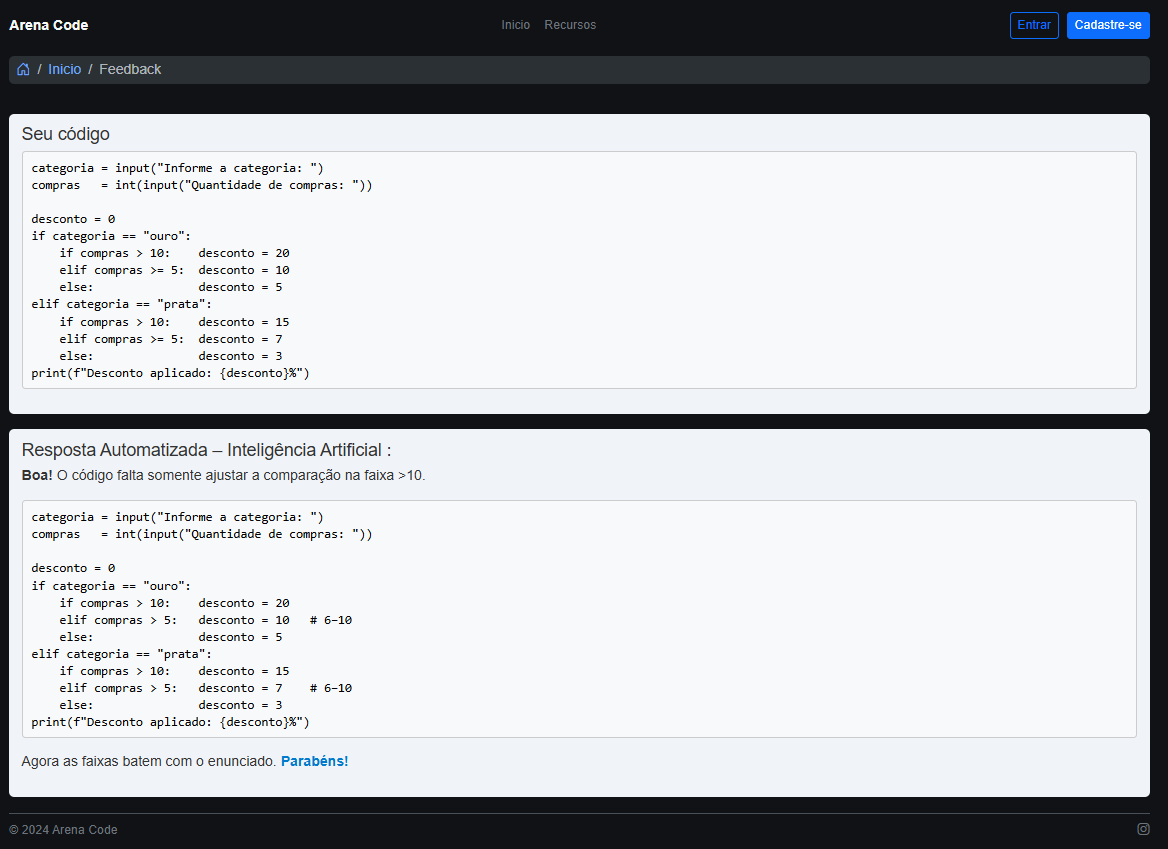
\includegraphics[width=14cm]{./imagens/capitulo7/ferramenta-fig3}
	\caption{Tela de Feedback (Elaboração própria, 2025) }
	\label{fig:ferramenta-fedback}
\end{figure}


Para realizar essa análise, a ferramenta monta um prompt com apenas duas entradas : o enunciado da questão e o código submetido. E posteriormente envia ao GPT-4. O modelo executa os casos de testes, identifica eventuais erros e devolve um feedback ao aluno. Esse ciclo tem como objetivo promover o aprimoramento contínuo, pois o aluno pode revisar e reenviar sua solução quantas vezes forem necessárias até alcançar o resultado desejado.  Para torná-lo utilizável pela interface, o sistema executa o seguinte prompt: 

\subsubsection{Entradas}

\begin{itemize}
    \item \textbf{Questão}: Enunciado da questão de programação que o estudante deve resolver.
    \item \textbf{Código submetido}: Código-fonte enviado pelo estudante como tentativa de solução.
\end{itemize}

\subsubsection{Prompt Enviado ao API do ChatGPT:}

"Você é um assistente especializado em revisar código e dar feedback aos alunos. Se minha resposta estiver errada explique exatamente onde errei, baseado na [\textbf{Questão}] e no [\textbf{Código submetido}], corrija a resposta de forma didática e dê uma resposta detalhada."


\section{Vantagens e limitações do modelo multicamadas}

Embora a configuração inicial dos templates exija um certo esforço de elaboração, esse investimento é compensado pela possibilidade de reutilizar as questões em diversas situações, reduzindo a necessidade de criar novos problemas para cada turma ou semestre. Uma vez que o repositório de problemas e cenários esteja consolidado, os professores podem extrair diferentes conjuntos de exercícios de forma rápida, adequando-os a diferentes turmas, níveis de dificuldade ou contextos de aplicação. A prática frequente com casos variados também permite aos estudantes um aprendizado mais consistente, pois eles entram em contato com diversas nuances do uso das estruturas condicionais, refinando sua capacidade de resolução de problemas, isto também se aplica a todo contexto que seja possível incluir vários cenários diferentes para um mesmo problema. No entanto, a mesma particularidade que torna o modelo efetivo também introduz algumas dificuldades tais como a manutenção de múltiplas camadas pode ser complexa sem ferramentas de apoio, e a qualidade das respostas depende diretamente da clareza dos \emph{prompts}. Para resumir esses pontos, a Tabela~\ref{tab:beneficios-limitacoes} apresenta um comparativo entre os principais benefícios observados e as limitações identificadas durante o desenvolvimento deste trabalho.


\begin{table}[H]
\centering
\caption{Comparativo de benefícios e limitações do modelo multicamadas}
\label{tab:beneficios-limitacoes}
\begin{tabular}{|p{7cm}|p{7cm}|}
\hline
\textbf{Benefícios} & \textbf{Limitações / Dificuldades} \\ \hline
\begin{itemize}[leftmargin=*]
    \item \textbf{Reutilização eficiente:} um único template pode gerar centenas de variações, reduzindo o esforço contínuo de elaboração de novos exercícios.%
    \item \textbf{Escalonamento:} permite calibrar o nível de dificuldade ou o contexto sem recriar todo o enunciado, respondendo rapidamente a diferentes perfis de turma.%
    \item \textbf{Facilita a manutenção:} ajustes conceituais (erros, melhorias, mudança de nomenclatura) são feitos apenas no template central.%
    \item \textbf{Feedback em tempo real:} integração direta com \textit{APIs} de IA (GPT-4) fornece correções detalhadas e adaptativas, incentivando múltiplas tentativas.%
    \item \textbf{Clareza para o professor:} separação explícita entre \emph{estrutura} e \emph{instâncias} torna o repositório de questões mais organizado e auditável.%
\end{itemize} &
\begin{itemize}[leftmargin=*]
    \item \textbf{Curva de aprendizagem inicial:} modelar corretamente as camadas demanda planejamento e domínio de variáveis, o que pode desestimular docentes sem familiaridade com templates.%
    \item \textbf{Ausência de interface gráfica:} editar arquivos JSON manualmente é suscetível a erros de sintaxe e aumenta o tempo de configuração; uma GUI dedicada ainda é necessária.%
    \item \textbf{Depuração complexa:} quando múltiplas camadas interagem, localizar inconsistências (e.g.\ índices trocados) pode ser trabalhoso.%
    \item \textbf{Limitações de mídia:} o modelo funciona muito bem para textos e números, mas não lida igualmente bem com variações de imagens, exigindo adaptações extras.%
    \item \textbf{Dependência de \textit{prompts} precisos:} erros na formulação do prompt para o GPT-4 geram feedback incoerente; não há controle total sobre a aleatoriedade das respostas.%
\end{itemize} \\ \hline
\end{tabular}
\end{table}


Com esse resultado podemos responder parcialmente à \textbf{QP1}. Esses pontos formam a base para o capítulo seguinte, onde será apresentado um estudo de caso com professores que ensinam programação, e como as vantagens se concretizam na prática e até que ponto os desafios podem ser amenizados. Só então será possível responder totalmente à \textbf{QP1} e \textbf{QP3}, avaliando o impacto real desta abordagem.

